\documentclass[11pt]{article}
\usepackage[margin=1in]{geometry}
\usepackage[utf8]{inputenc}
\usepackage[T1]{fontenc}
\usepackage{amsmath,amssymb}
\usepackage{booktabs}
\usepackage{enumitem}
\usepackage{tikz}
\usetikzlibrary{arrows.meta,positioning,trees}
\usepackage[hidelinks]{hyperref}

\newcommand{\ARSnode}[1]{%
  \node[circle,draw,minimum size=7mm,inner sep=0pt] (#1) {$#1$};%
}
\newcommand{\ARSnodeat}[2]{%
  \node[circle,draw,minimum size=7mm,inner sep=0pt, #2] (#1) {$#1$};%
}
\tikzset{
  >={Stealth[length=3mm]},
  every loop/.style={looseness=7},
  ptree/.style={level distance=10mm, sibling distance=18mm},
  nt/.style   ={draw, rounded corners, inner sep=1.2pt, font=\footnotesize\ttfamily, fill=gray!10},
  tm/.style   ={font=\footnotesize\ttfamily}
}

\title{CPSC-354 Report}
\author{Ray Hettleman \\ Chapman University \\ \texttt{rhettleman@chapman.edu}}
\date{September 2, 2025}

\begin{document}
\maketitle

\begin{abstract}
This report collects my weekly notes, homework, and reflections for CPSC-354. 
\end{abstract}

\tableofcontents
\newpage

% =========================================================
\section{Introduction}
This section intentionally left blank for now.

% =========================================================
\section{Week by Week}

% ---------- Week 1 ----------
\subsection{Week 1}

\subsubsection{Notes and Exploration}
We studied the MIU system from Hofstadter’s \emph{Gödel, Escher, Bach}. The task was to decide whether the string \texttt{MIII} can be derived from \texttt{MI} using the system’s rules.

\subsubsection{Homework}
\textbf{Rules.}
\begin{enumerate}[label=\Roman*.]
  \item If a string ends with \texttt{I}, you may append \texttt{U}.
  \item From \texttt{Mx} you may infer \texttt{Mxx}.
  \item Replace any occurrence of \texttt{III} by \texttt{U}.
  \item Delete any occurrence of \texttt{UU}.
\end{enumerate}

\textbf{Reasoning.}  
We begin with \texttt{MI}.  
Rule I allows \texttt{MIU}.  
Rule II doubles the sequence after \texttt{M}: \texttt{MI} $\Rightarrow$ \texttt{MII}, then \texttt{MIIII}, etc.  
Rule III can only replace consecutive \texttt{III} with a \texttt{U}.  
But because doubling produces powers of two \texttt{I}'s (1, 2, 4, 8, ...), 
we never get exactly three \texttt{I}'s.  
Thus, no sequence of rules produces \texttt{MIII}.  

\textbf{Conclusion.}  
It is impossible to derive \texttt{MIII} from \texttt{MI}.  
The parity of the number of \texttt{I}'s (always even after the first doubling) prevents reaching 3.

\subsubsection{Questions}
\emph{What is a rule that could be implemented that, while still requiring many steps, makes the MU-Puzzle solvable?}

% ---------- Week 2 ----------
\subsection{Week 2}

\subsubsection{Notes and Exploration}
We explored Abstract Reduction Systems (ARS), focusing on termination, confluence, and unique normal forms (UNFs). 
Each ARS was represented as a graph, and we determined its key properties.

\subsubsection{Homework}
\paragraph{1.\; $A=\varnothing$}
No nodes or edges.  
Terminating: True. Confluent: True. UNFs: True.

\paragraph{2.\; $A=\{a\},\; R=\varnothing$}
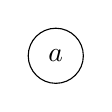
\begin{tikzpicture}
  \ARSnode{a};
\end{tikzpicture}

Normal forms: $a$. Terminating: True. Confluent: True. UNFs: True.

\paragraph{3.\; $A=\{a\},\; R=\{(a,a)\}$}
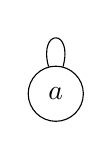
\begin{tikzpicture}
  \ARSnode{a};
  \path (a) edge[loop above] (a);
\end{tikzpicture}

Infinite sequence $a\to a\to\cdots$.  
Terminating: False. Confluent: True. UNFs: False.

\paragraph{4.\; $A=\{a,b,c\},\; R=\{(a,b),(a,c)\}$}
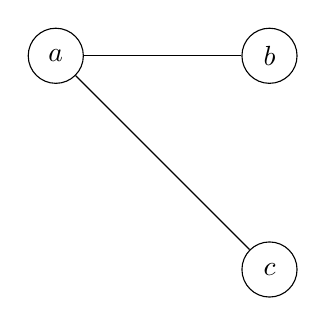
\begin{tikzpicture}[node distance=20mm]
  \ARSnode{a};
  \ARSnodeat{b}{right=of a}
  \ARSnodeat{c}{below=of b}
  \draw (a) edge (b) (a) edge (c);
\end{tikzpicture}

$b$ and $c$ are normal forms, so from $a$ two distinct endpoints are reachable.  
Terminating: True. Confluent: False. UNFs: False.

\paragraph{5.\; $A=\{a,b\},\; R=\{(a,a),(a,b)\}$}
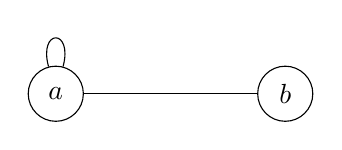
\begin{tikzpicture}[node distance=22mm]
  \ARSnode{a};
  \ARSnodeat{b}{right=of a}
  \draw (a) edge[loop above] (a) (a) edge (b);
\end{tikzpicture}

$b$ is normal; all paths from $a$ can reach $b$.  
Terminating: False. Confluent: True. UNFs: True.

\paragraph{6.\; $A=\{a,b,c\},\; R=\{(a,b),(b,b),(a,c)\}$}
\begin{tikzpicture}[node distance=22mm]
  \ARSnode{a};
  \ARSnodeat{b}{right=of a}
  \ARSnodeat{c}{below=of b}
  \draw (a) edge (b) (a) edge (c) (b) edge[loop above] (b);
\end{tikzpicture}

Non-terminating through $b\to b$; $c$ is normal but unreachable from $b$.  
Terminating: False. Confluent: False. UNFs: False.

\paragraph{7.\; $A=\{a,b,c\},\; R=\{(a,b),(b,b),(a,c),(c,c)\}$}
\begin{tikzpicture}[node distance=22mm]
  \ARSnode{a};
  \ARSnodeat{b}{right=of a}
  \ARSnodeat{c}{below=of b}
  \draw (a) edge (b) (a) edge (c) (b) edge[loop above] (b) (c) edge[loop right] (c);
\end{tikzpicture}

Both $b$ and $c$ loop indefinitely.  
Terminating: False. Confluent: False. UNFs: False.

\textbf{Summary Table:}
\begin{center}
\begin{tabular}{@{}clccc@{}}
\toprule
\# & $(A,R)$ & confluent & terminating & unique NFs \\
\midrule
1 & $(\varnothing,\varnothing)$ & True & True & True \\
2 & $(\{a\},\varnothing)$ & True & True & True \\
3 & $(\{a\},\{(a,a)\})$ & True & False & False \\
4 & $(\{a,b,c\},\{(a,b),(a,c)\})$ & False & True & False \\
5 & $(\{a,b\},\{(a,a),(a,b)\})$ & True & False & True \\
6 & $(\{a,b,c\},\{(a,b),(b,b),(a,c)\})$ & False & False & False \\
7 & $(\{a,b,c\},\{(a,b),(b,b),(a,c),(c,c)\})$ & False & False & False \\
\bottomrule
\end{tabular}
\end{center}

\textbf{All 8 Combinations:}
\begin{center}
\begin{tabular}{@{}ccccl@{}}
\toprule
confluent & terminating & unique NFs & example \\
\midrule
True  & True  & True  & ARS 2 (or 1) \\
True  & True  & False  & \textit{Impossible} \\
True  & False  & True  & ARS 5 \\
True  & False  & False  & ARS 3 \\
False & True  & True  & \textit{Impossible} \\
False & True  & False  & ARS 4 \\
False & False & True  & \textit{Impossible} \\
False & False & False & ARS 6 (or 7) \\
\bottomrule
\end{tabular}
\end{center}

\subsubsection{Questions}
\emph{Is there an easy way to tell from the graph if an ARS will terminate, or do you always have to trace every path?}

% ---------- Week 3 ----------
\subsection{Week 3}

\subsubsection{Notes and Exploration}
Exercises 5 and 5b extended ARS analysis with additional looping rules.

\subsubsection{Homework}
\textbf{Exercise 5.}  
$A=\{a,b\}$ with $a\to a$, $a\to b$.  
Loop $a\to a$ means not terminating, but since all paths eventually lead to $b$, the system is confluent with a unique NF.

\textbf{Exercise 5b.}  
Add $c$ with $a\to c$, $c\to c$.  
Now one branch terminates ($b$) and the other loops, breaking confluence.

\subsubsection{Questions}
\emph{Could we make a version of 5b that still loops but somehow keeps unique normal forms?}

% ---------- Week 4 ----------
\subsection{Week 4}

\subsubsection{Notes and Exploration}
We introduced termination proofs and measure functions.

\subsubsection{Homework}
\paragraph{HW 4.1 (Euclidean Algorithm).}
\begin{verbatim}
while b != 0:
  temp = b
  b = a mod b
  a = temp
return a
\end{verbatim}
This algorithm terminates when $b>0$ because $b$ decreases with each iteration.  
The measure function $m(a,b)=b$ is always non-negative and strictly decreases.

\paragraph{HW 4.2 (Merge Sort).}
\begin{verbatim}
function merge_sort(arr, left, right):
  if left >= right: return
  mid = (left + right) / 2
  merge_sort(arr, left, mid)
  merge_sort(arr, mid+1, right)
  merge(arr, left, mid, right)
\end{verbatim}
The measure $\varphi(left,right)=right-left+1$ decreases with every recursive call.  
When it reaches 1, the recursion stops, proving termination.

\subsubsection{Questions}
\emph{What would it look like to design a sorting algorithm that checks to see if an input is terminating?}

% ---------- Week 5 ----------
\subsection{Week 5}

\subsubsection{Notes and Exploration}
We practiced $\lambda$-calculus reduction and substitution.

\subsubsection{Homework}
Evaluate:
\[
  (\lambda f.\lambda x.f(f(x)))\,(\lambda f.\lambda x.f(f(f(x)))).
\]

\textbf{Step 1.} Parentheses group left:  
\[
  ((\lambda f.\lambda x.f(f(x)))(\lambda f.\lambda x.f(f(f(x))))).
\]

\textbf{Step 2.} Apply $\beta$-reduction:  
\[
  \mapsto \lambda x.(\lambda f.\lambda x.f(f(f(x))))((\lambda f.\lambda x.f(f(f(x))))x).
\]

\textbf{Step 3.} Rename inner $x\to y$ and reduce:  
\[
  (\lambda f.\lambda y.f(f(f(y))))x \mapsto \lambda y.x(x(x(y))).
\]

\textbf{Step 4.} Apply again:  
\[
  \lambda x.\lambda y.x^9(y).
\]

\textbf{Conclusion.}  
The function composes $f$ twice and $f^3$ thrice, resulting in a ninefold application.

\subsubsection{Questions}
\emph{What would happen if we swapped the two functions in the workout?}

% ---------- Week 6 ----------
\subsection{Week 6}

\subsubsection{Notes and Exploration}
We computed factorial using the fixed-point combinator \texttt{fix}.

\subsubsection{Homework}
Compute:
\[
\texttt{let rec fact = \textbackslash n. if n=0 then 1 else n * fact (n-1) in 3}
\]
Using the rules:
\[
\texttt{fix F $\mapsto$ F (fix F)}, \quad
\texttt{let rec f = e1 in e2 $\mapsto$ let f = (fix (\textbackslash f.e1)) in e2}.
\]
We unfold recursively:
\[
\texttt{fact 3 $\mapsto$ 3 * (fix F) 2 $\mapsto$ 3 * 2 * 1 = 6}.
\]

\textbf{Conclusion.}  
Following only the allowed computation rules, \texttt{fact 3} reduces to \textbf{6}.

\subsubsection{Questions}
\emph{Would using $\alpha$-conversion anywhere in the factorial example change the result, or just make it cleaner?}

% ---------- Week 7 ----------
\subsection{Week 7}

\subsubsection{Notes and Exploration}
Parsing and context-free grammars. We use the grammar (nonterminals \texttt{Exp}, \texttt{Exp1}, \texttt{Exp2}):

\begin{verbatim}
Exp  -> Exp '+' Exp1
Exp1 -> Exp1 '*' Exp2
Exp2 -> Integer
Exp2 -> '(' Exp ')'
Exp  -> Exp1
Exp1 -> Exp2
\end{verbatim}

\subsubsection{Homework: Parse Trees}
Below are derivation trees (concrete syntax trees) for the required expressions. 
Nonterminals are boxed; terminals are leaves.

\paragraph{(a) \texttt{2+1}}
\begin{center}
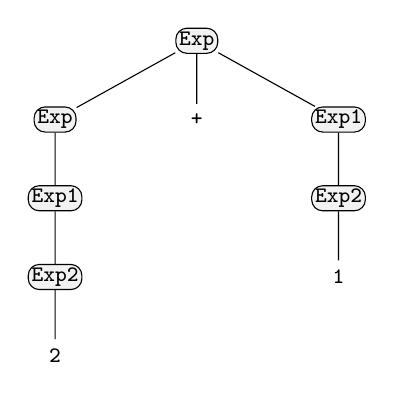
\begin{tikzpicture}[ptree]
\node[nt]{Exp}
  child { node[nt]{Exp}
    child { node[nt]{Exp1}
      child { node[nt]{Exp2}
        child { node[tm]{2} }
      }
    }
  }
  child { node[tm]{+} }
  child { node[nt]{Exp1}
    child { node[nt]{Exp2}
      child { node[tm]{1} }
    }
  };
\end{tikzpicture}
\end{center}

\paragraph{(b) \texttt{1+2*3}}
\begin{center}
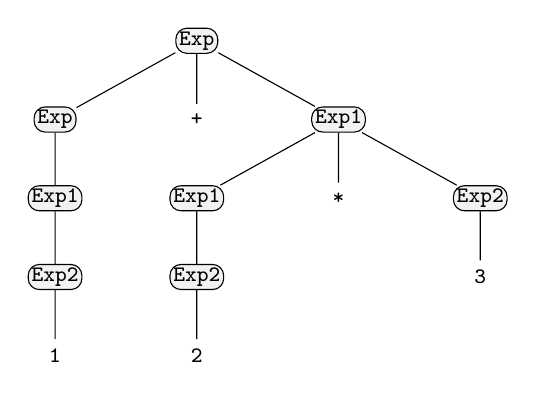
\begin{tikzpicture}[ptree]
\node[nt]{Exp}
  child { node[nt]{Exp}
    child { node[nt]{Exp1}
      child { node[nt]{Exp2}
        child { node[tm]{1} }
      }
    }
  }
  child { node[tm]{+} }
  child { node[nt]{Exp1}
    child { node[nt]{Exp1}
      child { node[nt]{Exp2} child { node[tm]{2} } }
    }
    child { node[tm]{*} }
    child { node[nt]{Exp2} child { node[tm]{3} } }
  };
\end{tikzpicture}
\end{center}

\paragraph{(c) \texttt{1+(2*3)}}
\begin{center}
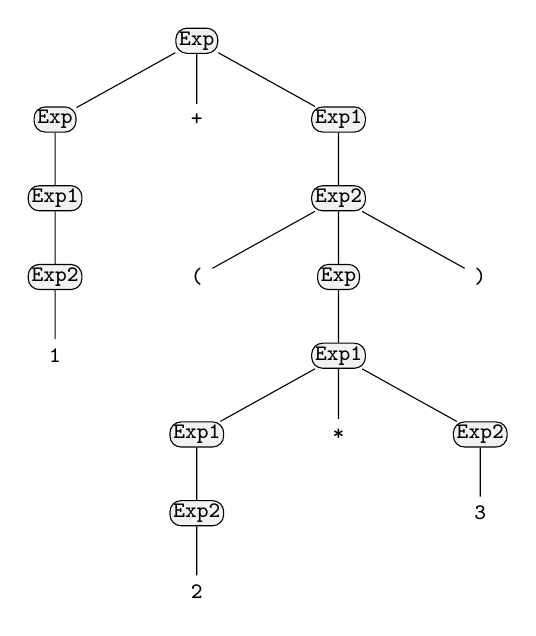
\begin{tikzpicture}[ptree]
\node[nt]{Exp}
  child { node[nt]{Exp}
    child { node[nt]{Exp1}
      child { node[nt]{Exp2} child { node[tm]{1} } }
    }
  }
  child { node[tm]{+} }
  child { node[nt]{Exp1}
    child { node[nt]{Exp2}
      child { node[tm]{(} }
      child { node[nt]{Exp}
        child { node[nt]{Exp1}
          child { node[nt]{Exp1}
            child { node[nt]{Exp2} child { node[tm]{2} } }
          }
          child { node[tm]{*} }
          child { node[nt]{Exp2} child { node[tm]{3} } }
        }
      }
      child { node[tm]{)} }
    }
  };
\end{tikzpicture}
\end{center}


\paragraph{(d) \texttt{(1+2)*3}}
\begin{center}
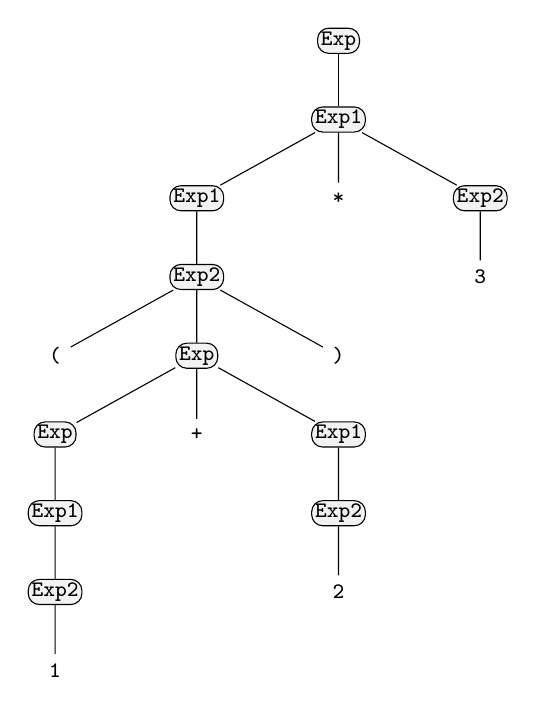
\begin{tikzpicture}[ptree]
\node[nt]{Exp}
  child { node[nt]{Exp1}
    child { node[nt]{Exp1}
      child { node[nt]{Exp2}
        child { node[tm]{(} }
        child { node[nt]{Exp}
          child { node[nt]{Exp}
            child { node[nt]{Exp1}
              child { node[nt]{Exp2} child { node[tm]{1} } }
            }
          }
          child { node[tm]{+} }
          child { node[nt]{Exp1}
            child { node[nt]{Exp2} child { node[tm]{2} } }
          }
        }
        child { node[tm]{)} }
      }
    }
    child { node[tm]{*} }
    child { node[nt]{Exp2} child { node[tm]{3} } }
  };
\end{tikzpicture}
\end{center}

\paragraph{(e) \texttt{1+2*3+4*5+6}}
\begin{center}
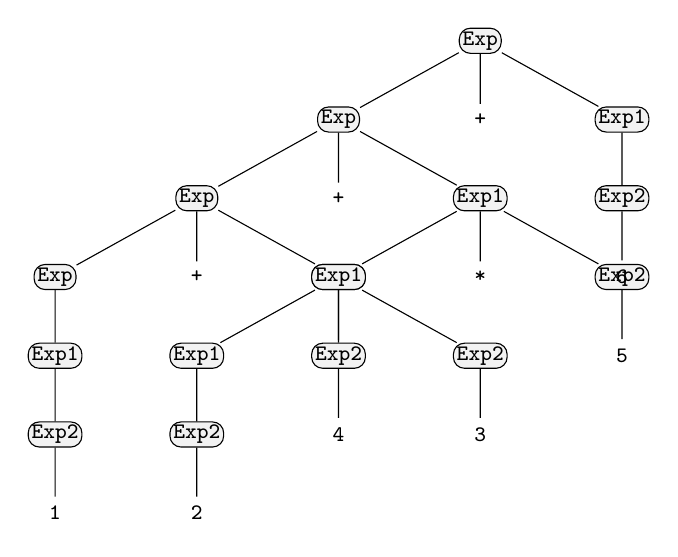
\begin{tikzpicture}[ptree]
\node[nt]{Exp}
  % Left: ((1 + 2*3) + 4*5)
  child { node[nt]{Exp}
    child { node[nt]{Exp}
      % (1 + 2*3)
      child { node[nt]{Exp}
        child { node[nt]{Exp1}
          child { node[nt]{Exp2} child { node[tm]{1} } }
        }
      }
      child { node[tm]{+} }
      child { node[nt]{Exp1}
        child { node[nt]{Exp1}
          child { node[nt]{Exp2} child { node[tm]{2} } }
        }
        child { node[tm]{*} }
        child { node[nt]{Exp2} child { node[tm]{3} } }
      }
    }
    child { node[tm]{+} }
    child { node[nt]{Exp1}
      child { node[nt]{Exp1}
        child { node[nt]{Exp2} child { node[tm]{4} } }
      }
      child { node[tm]{*} }
      child { node[nt]{Exp2} child { node[tm]{5} } }
    }
  }
  child { node[tm]{+} }
  child { node[nt]{Exp1}
    child { node[nt]{Exp2} child { node[tm]{6} } }
  };
\end{tikzpicture}
\end{center}

% =========================================================
\subsubsection{Questions}
\emph{Could this grammar still work if “+” and “” had the same priority?}

% ---------- Week 8 ----------
\subsection{Week 8}

\subsubsection{Notes and Exploration}
I completed Levels 5--8 of the \emph{Natural Number Game} (NNG). The key tools were:
\begin{itemize}[leftmargin=1.4em]
  \item \textbf{Rewriting} with \texttt{rw [lemma]} to substitute equals for equals.
  \item \textbf{\texttt{rfl}} to close a goal when both sides are definitionally identical.
  \item Peano-style equations for addition and numerals, including \texttt{add\_zero}, \texttt{add\_succ}, \texttt{add\_one}, \texttt{one\_eq\_succ\_zero}, and \texttt{two\_eq\_succ\_one}.
\end{itemize}

\subsubsection{Homework (NNG Levels 5--8)}
\paragraph{5/8: Adding zero.} \emph{Goal:} $a + (b+0) + (c+0) = a+b+c$.\\
\emph{Lean steps:} \texttt{rw [add\_zero]} (on $b+0$), \texttt{rw [add\_zero]} (on $c+0$), \texttt{rfl}.

\paragraph{6/8: Precision rewriting.} \emph{Goal:} $a + (b+0) + (c+0) = a+b+c$.\\
\emph{Lean steps:} \texttt{rw [add\_zero]} (on $b+0$), \texttt{rw [add\_zero]} (on $c+0$), \texttt{rfl}.

\paragraph{7/8: \texttt{add\_succ}.} \emph{Goal:} $\mathrm{succ}\,n = n+1$.\\
\emph{Lean steps:} \texttt{rw [one\_eq\_succ\_zero]} to get $n+1=n+\mathrm{succ}\,0$; \texttt{rw [add\_succ]} to obtain $\mathrm{succ}(n+0)$; \texttt{rw [add\_zero]}; \texttt{rfl}.

\paragraph{8/8: $2+2=4$.} \emph{Outline:} Rewrite $2$ and $4$ as successors (\texttt{two\_eq\_succ\_one}, etc.), use \texttt{add\_succ} to pull \(\mathrm{succ}\) out of addition stepwise, and finish by \texttt{rfl} once both sides match.

\subsubsection{Natural-Language Proof (English math proof)}
\paragraph{Claim.} \(2+2=4\).

\paragraph{Assumptions/Definitions.}
Let \(0\) be the base natural number and \(\mathrm{succ}(n)\) the successor of \(n\).
Define \(1=\mathrm{succ}(0)\), \(2=\mathrm{succ}(1)\), and \(4=\mathrm{succ}(\mathrm{succ}(\mathrm{succ}(\mathrm{succ}(0))))\).
Addition is defined by the Peano axioms:
\[
\forall a,\; a+0=a \quad\text{and}\quad \forall a,b,\; a+\mathrm{succ}(b)=\mathrm{succ}(a+b).
\]

\paragraph{Proof.}
We compute \(2+2\) using the addition axioms.
First rewrite \(2=\mathrm{succ}(1)\), so
\[
2+2 \;=\; 2+\mathrm{succ}(1) \;=\; \mathrm{succ}(2+1) \quad\text{(by the second axiom).}
\]
Again rewrite \(1=\mathrm{succ}(0)\) to get
\[
2+1 \;=\; 2+\mathrm{succ}(0) \;=\; \mathrm{succ}(2+0) \;=\; \mathrm{succ}(2) \quad\text{(using both axioms).}
\]
Therefore
\[
2+2 \;=\; \mathrm{succ}(2+1) \;=\; \mathrm{succ}(\mathrm{succ}(2)).
\]
Since \(2=\mathrm{succ}(1)\), we have
\[
\mathrm{succ}(\mathrm{succ}(2))=\mathrm{succ}(\mathrm{succ}(\mathrm{succ}(1)))=
\mathrm{succ}(\mathrm{succ}(\mathrm{succ}(\mathrm{succ}(0))))=4.
\]
Hence \(2+2=4\). \(\square\)

\subsubsection{Discord Question}
\emph{When using \texttt{rw [add\_zero]}, how does Lean know which part of the equation to rewrite first?}

% ---------- Week 9 ----------
\subsection{Week 9}

\subsubsection{Notes and Exploration}
This week I worked through \emph{Addition World} in the Natural Number Game.  
Key theorems proved in this world:
\begin{itemize}[leftmargin=1.4em]
  \item \textbf{zero\_add:} $0 + n = n$ (proved by induction).
  \item \textbf{succ\_add:} $\mathrm{succ}(a) + b = \mathrm{succ}(a + b)$ (proved by induction).
  \item \textbf{add\_comm:} $a + b = b + a$ (commutativity of $+$).
  \item \textbf{add\_assoc:} $(a + b) + c = a + (b + c)$ (associativity of $+$).
  \item \textbf{add\_right\_comm:} $(a + b) + c = (a + c) + b$.
\end{itemize}

The HW 9 instruction is:  
For Level 5 of addition world (\texttt{add\_right\_comm}), give two solutions in the report:
(1) a proof that uses induction and  
(2) a proof that does \emph{not} use induction.  
For each version, also write the corresponding ``pen-and-paper'' math proof.

\subsubsection{Homework (Addition World Level 5 / HW 9)}

\paragraph{Theorem (Level 5).}
For all natural numbers $a,b,c$, we have
\[
(a + b) + c \;=\; (a + c) + b.
\]
In Lean, this theorem is called \texttt{add\_right\_comm}.

\bigskip
\noindent\textbf{Solution A: With Induction.}  
We prove \texttt{add\_right\_comm} by induction on $c$.

\emph{Lean tactic steps:}
\begin{itemize}[leftmargin=1.4em]
  \item \texttt{induction c with d hd}
  \item \texttt{rw [add\_zero]}
  \item \texttt{rw [add\_zero]}
  \item \texttt{rfl}
  \item \texttt{rw [add\_succ]}
  \item \texttt{rw [succ\_add]}
  \item \texttt{rw [hd]}
  \item \texttt{rfl}
\end{itemize}

Explanation of structure (what the tactics are doing, summarized in math terms):

\emph{Base case ($c=0$).}  
Goal:
\[
(a+b)+0 \;=\; (a+0)+b.
\]
By \texttt{add\_zero}, $(a+b)+0 = a+b$, and $(a+0)+b = a+b$.  
So both sides are $a+b$. Closed by \texttt{rfl}.

\emph{Inductive step ($c = \mathrm{succ}(d)$).}  
Induction hypothesis (called \texttt{hd} in Lean):
\[
(a+b)+d \;=\; (a+d)+b.
\]
Goal:
\[
(a+b)+\mathrm{succ}(d) \;=\; (a+\mathrm{succ}(d))+b.
\]

Using the Peano definition of $+$ on the right argument,
\[
(a+b)+\mathrm{succ}(d) = \mathrm{succ}((a+b)+d)
\quad\text{and}\quad
a+\mathrm{succ}(d) = \mathrm{succ}(a+d).
\]
So the right-hand side becomes
\[
(a+\mathrm{succ}(d))+b
= (\mathrm{succ}(a+d))+b
= \mathrm{succ}\big((a+d)+b\big)
\]
using \texttt{succ\_add}, which says $\mathrm{succ}(x)+y=\mathrm{succ}(x+y)$.

Thus the goal reduces to
\[
\mathrm{succ}\big((a+b)+d\big)
=
\mathrm{succ}\big((a+d)+b\big).
\]
By the induction hypothesis, $(a+b)+d = (a+d)+b$, so the two $\mathrm{succ}(\cdot)$ terms are equal. This closes with \texttt{rfl}.

\emph{Conclusion.}  
By induction on $c$, $(a+b)+c = (a+c)+b$ holds for all $a,b,c$.

\bigskip
\noindent\textbf{Solution B: Without Induction.}  
We can also prove \texttt{add\_right\_comm} using only associativity and commutativity of addition, without \texttt{induction}.

\emph{Lean tactic steps (no induction):}
\begin{itemize}[leftmargin=1.4em]
  \item \texttt{rw [add\_assoc]}
  \item \texttt{rw [add\_comm b c]}
  \item \texttt{rw [\textbackslash leftarrow{} add\_assoc]}
  \item \texttt{rfl}
\end{itemize}

Those steps correspond exactly to the following algebra moves:
\[
(a+b)+c
\;=\;
a+(b+c)
\quad\text{(associativity, \texttt{add\_assoc})}
\]
\[
=\;
a+(c+b)
\quad\text{(commutativity on $b+c$, \texttt{add\_comm b c})}
\]
\[
=\;
(a+c)+b
\quad\text{(associativity again, undoing \texttt{add\_assoc})}.
\]
This matches the goal $(a+b)+c = (a+c)+b$.

\bigskip
\noindent\textbf{English/Pen-and-Paper Proofs for HW 9}

\paragraph{Solution A (Induction Proof in Math).}
We prove $(a+b)+c = (a+c)+b$ for all $a,b,c \in \mathbb{N}$ by induction on $c$.

\textbf{Base case:} $c=0$.  
Then
\[
(a+b)+0 = a+b
\quad\text{and}\quad
(a+0)+b = a+b,
\]
because $x+0=x$ for any $x$.  
So $(a+b)+0 = (a+0)+b$.

\textbf{Inductive step:} Assume $(a+b)+d = (a+d)+b$ for some $d$.  
We must show $(a+b)+\mathrm{succ}(d) = (a+\mathrm{succ}(d))+b$.

By the Peano definition of addition on the right argument,
\[
(a+b)+\mathrm{succ}(d) = \mathrm{succ}((a+b)+d).
\]
Also,
\[
a+\mathrm{succ}(d) = \mathrm{succ}(a+d),
\]
so
\[
(a+\mathrm{succ}(d))+b 
= (\mathrm{succ}(a+d))+b 
= \mathrm{succ}((a+d)+b),
\]
using the lemma $\mathrm{succ}(x)+y = \mathrm{succ}(x+y)$.

So it suffices to show
\[
\mathrm{succ}((a+b)+d) = \mathrm{succ}((a+d)+b),
\]
which follows from the induction hypothesis $(a+b)+d = (a+d)+b$.  
Therefore the statement holds for $\mathrm{succ}(d)$.

By induction on $c$, $(a+b)+c = (a+c)+b$ for all $a,b,c$.

\paragraph{Solution B (Algebraic / No Induction).}
We use associativity and commutativity of addition on $\mathbb{N}$.

Starting from the left-hand side,
\[
(a+b)+c = a+(b+c)
\quad\text{(associativity of $+$)},
\]
\[
= a+(c+b)
\quad\text{(commutativity of $+$)},
\]
\[
= (a+c)+b
\quad\text{(associativity of $+$ again)}.
\]
This is exactly the desired right-hand side $(a+c)+b$.  
No induction was needed.

\subsubsection{Questions}
\emph{When should I solve these problems using induction vs without?}

% =========================================================
\section{Essay (Synthesis)}
This section intentionally left blank.

% =========================================================
\section{Evidence of Participation}
This section intentionally left blank.

% =========================================================
\section{Conclusion}
This section intentionally left blank.

% =========================================================
\section*{References}


\end{document}
